\subsection{Гравитационное линзирование}

\term{Гравитационное линзирование}~--- эффект, связанный с искривлением распространения электромагнитного излучения гравитационным полем массивного тела или системы тел (галактик, скопления галактик, скопления тёмной материи).

На (Рис.~\ref{grav-lens}) показано, как происходит гравитационное линзирование. $S$~--- источник электромагнитных волн, $O$~--- наблюдатель, $J_1$ и $J_2$~--- видимые положения источника, $M$~--- массивное тело.

\begin{figure}[h!]
	\centering
	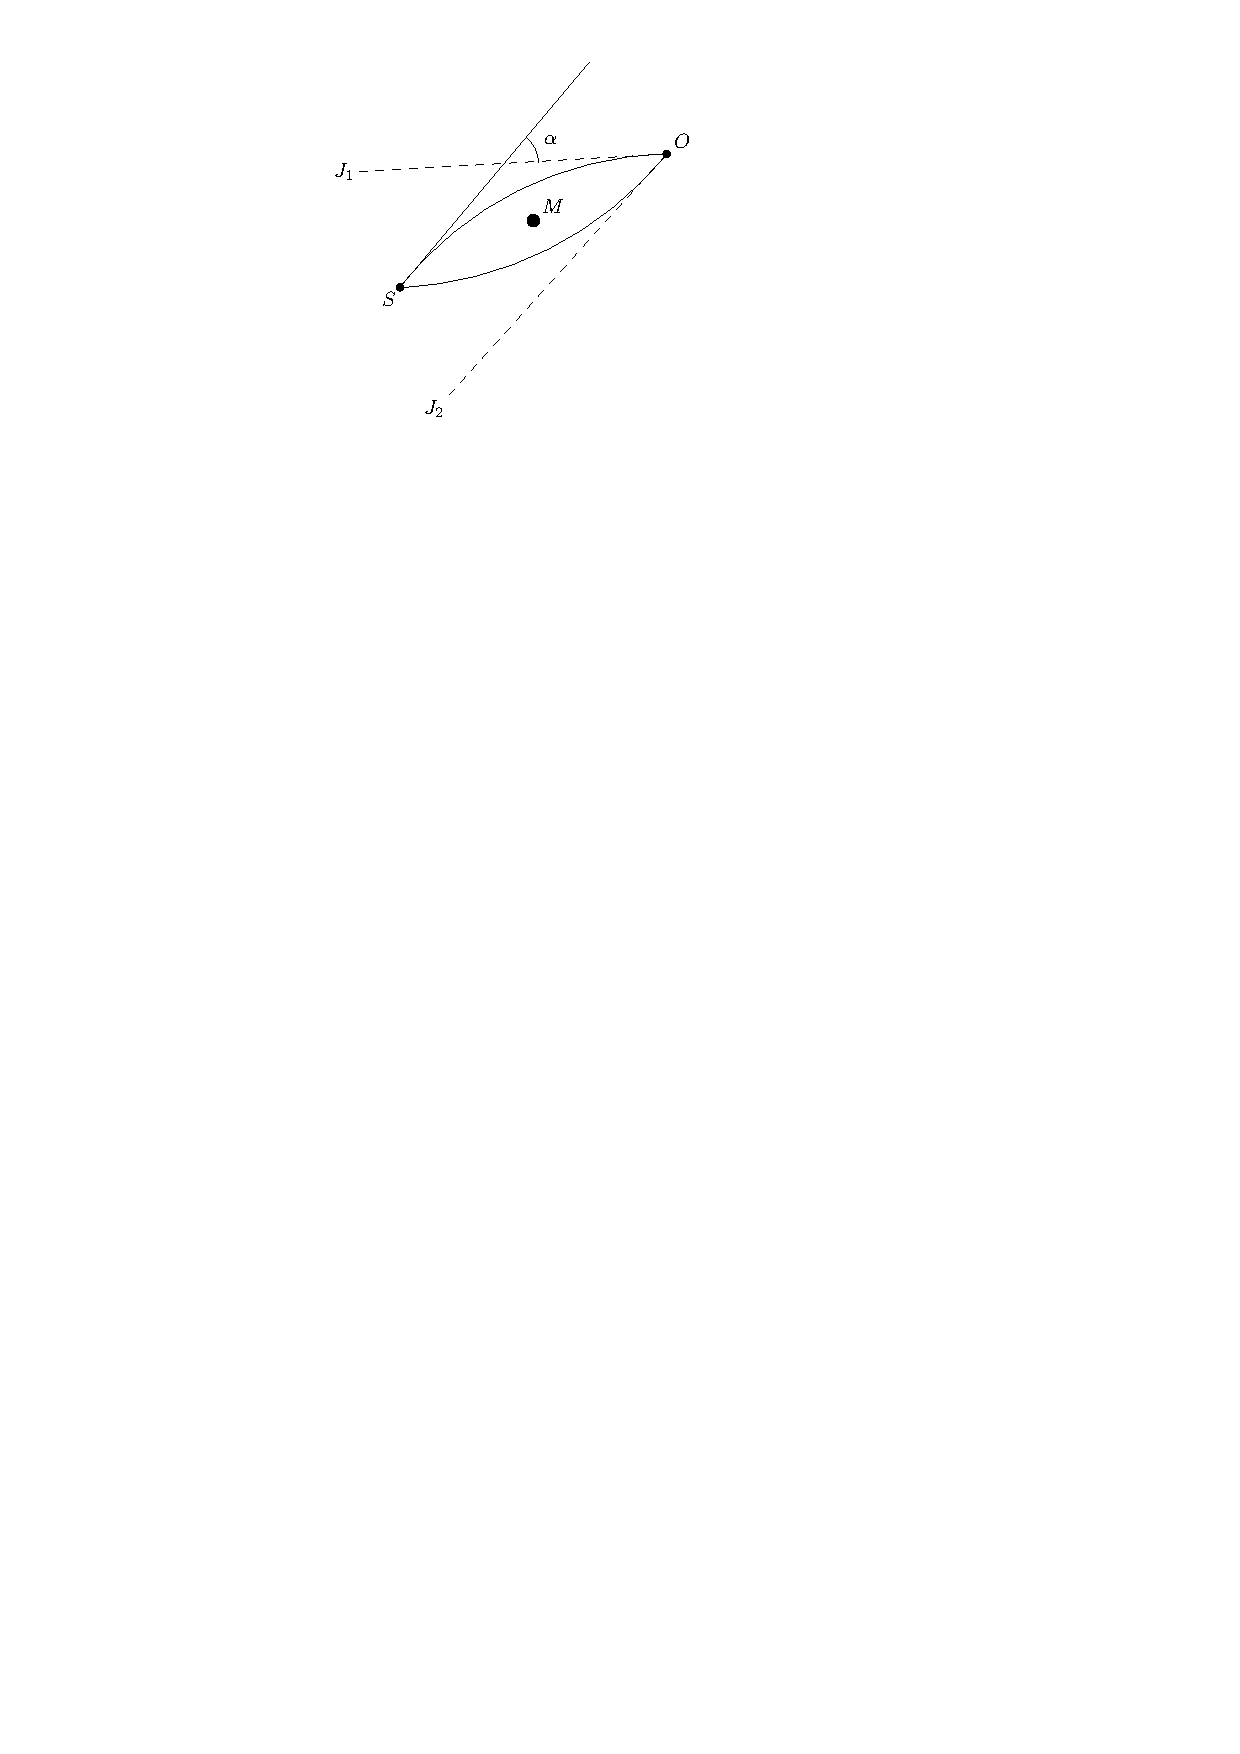
\includegraphics[width=0.4\tw]{grav-lens}
	\caption{Гравитационное линзирование}
	\label{grav-lens}
\end{figure}

Для угла преломления лучей в ходе гравитационного линзирования справедлива следующая формула: \begin{equation}
	\alpha = \frac{4 G M}{R c^2},
\end{equation}
где $M$~--- масса тела, отклоняющего луч, $R$~--- радиус этого тела, $c$~--- скорость света.